\documentclass[border=5pt]{standalone}
\usepackage[T1]{fontenc}
\usepackage{tikz}

\definecolor{horseshoe}{HTML}{65780B}
\definecolor{atlantic}{HTML}{466A9F}
\definecolor{garnet}{HTML}{73000A}
\definecolor{rose}{HTML}{CC2E40}
\definecolor{warmgrey}{HTML}{676156}

\begin{document}
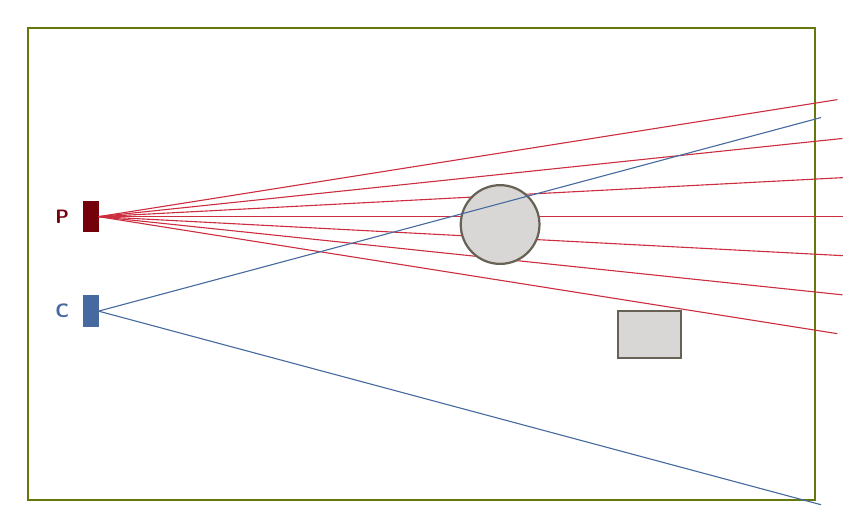
\begin{tikzpicture}
  \useasboundingbox (-3,-3) rectangle (7,3);
  \draw[horseshoe, thick] (-3,-3) rectangle (7,3);

  % ── Projector (left, slightly above center) ──
  \fill[garnet] (-2.3,0.4) rectangle (-2.1,0.8);
  \node[font=\scriptsize\sffamily\bfseries, color=garnet, left] at (-2.35,0.6) {P};

  % ── Camera (left, slightly below center) ──
  \fill[atlantic] (-2.3,-0.8) rectangle (-2.1,-0.4);
  \node[font=\scriptsize\sffamily\bfseries, color=atlantic, left] at (-2.35,-0.6) {C};

  % ── Projected stripes (top-down: fan of lines going right) ──
  % Evenly spaced lines from projector, fanning slightly
  \foreach \i in {-3,...,3} {
    \pgfmathsetmacro{\ang}{\i * 3}
    \draw[rose, thin] (-2.1,0.6) -- ++(\ang:9.5);
  }

  % ── Objects in scene (top-down shapes) ──
  % Circle
  \fill[warmgrey!25] (3,0.5) circle (0.5);
  \draw[warmgrey, thick] (3,0.5) circle (0.5);

  % Rectangle
  \fill[warmgrey!25] (4.5,-1.2) rectangle (5.3,-0.6);
  \draw[warmgrey, thick] (4.5,-1.2) rectangle (5.3,-0.6);

  % Camera FOV (observing the scene from below-left)
  \draw[atlantic, thin] (-2.1,-0.6) -- ++(15:9.5);
  \draw[atlantic, thin] (-2.1,-0.6) -- ++(-15:9.5);

\end{tikzpicture}
\end{document}
